
%  \section{The PSF profile analysis}

Since the complex 6-parameter PSF fit given by Eq.~(\ref{eq:SDSSPSF}) was adopted by 
the SDSS processing pipeline, significant progress has been made in validating the 
\vk~model of the atmosphere and measuring the associated outer
scale (see, for example, \citealt{Tokovinin2002}, \citealt{Boccas2004}, and \citealt{MartinezMessenger}).
In this section, we describe our much simpler 2-parameter fits to the SDSS PSF
profiles using the \vk~atmosphere model.

Our fitting of each PSF profile is a 2-step process. First we fit the
measured PSF profile to a \vk~PSF, with only one free parameter -
the FWHM of the \vk~profile.  The \vk~PSF profile is generated by creating the atmosphere
structure function first, as given by Eq. (18) in \cite{Tokovinin2002}, then calculating the
PSF through the Optical Transfer Function. 
The radial profiles of the \vk~PSF with a few different values of
outer scale is shown in Fig.~\ref{fig:vonK}.
The shape variation due to uncertainty in the outer scale, $L_0$, is seen to
be small. In this work, we have assumed a fiducial outer scale of 30 meters.
The impact of the exact value of $L_0$ is small, as illustrated in Fig.~\ref{fig:vonK}. 
We note that a fixed value of $L_0$ induces a small systematic uncertainty in 
the normalization of the contribution of instrumental PSF, discussed in \S~\ref{sec:instrPSF} 
below. 

Ideally, the Fried parameter $r_0$ would be used as the free
parameter in the fit to the \vk~model. However, 
that would require us to calculate the special functions and do the
Fourier Transform on a large array for each function evaluation.
Instead, we opted to generate a single \vk~PSF template with the FWHM of 
1 arcsec. In our one-parameter \vk~fit, we only stretch or compress
the template radially to get the best match with the data, in the
least-square sense.

\begin{figure}[ht]
\centering
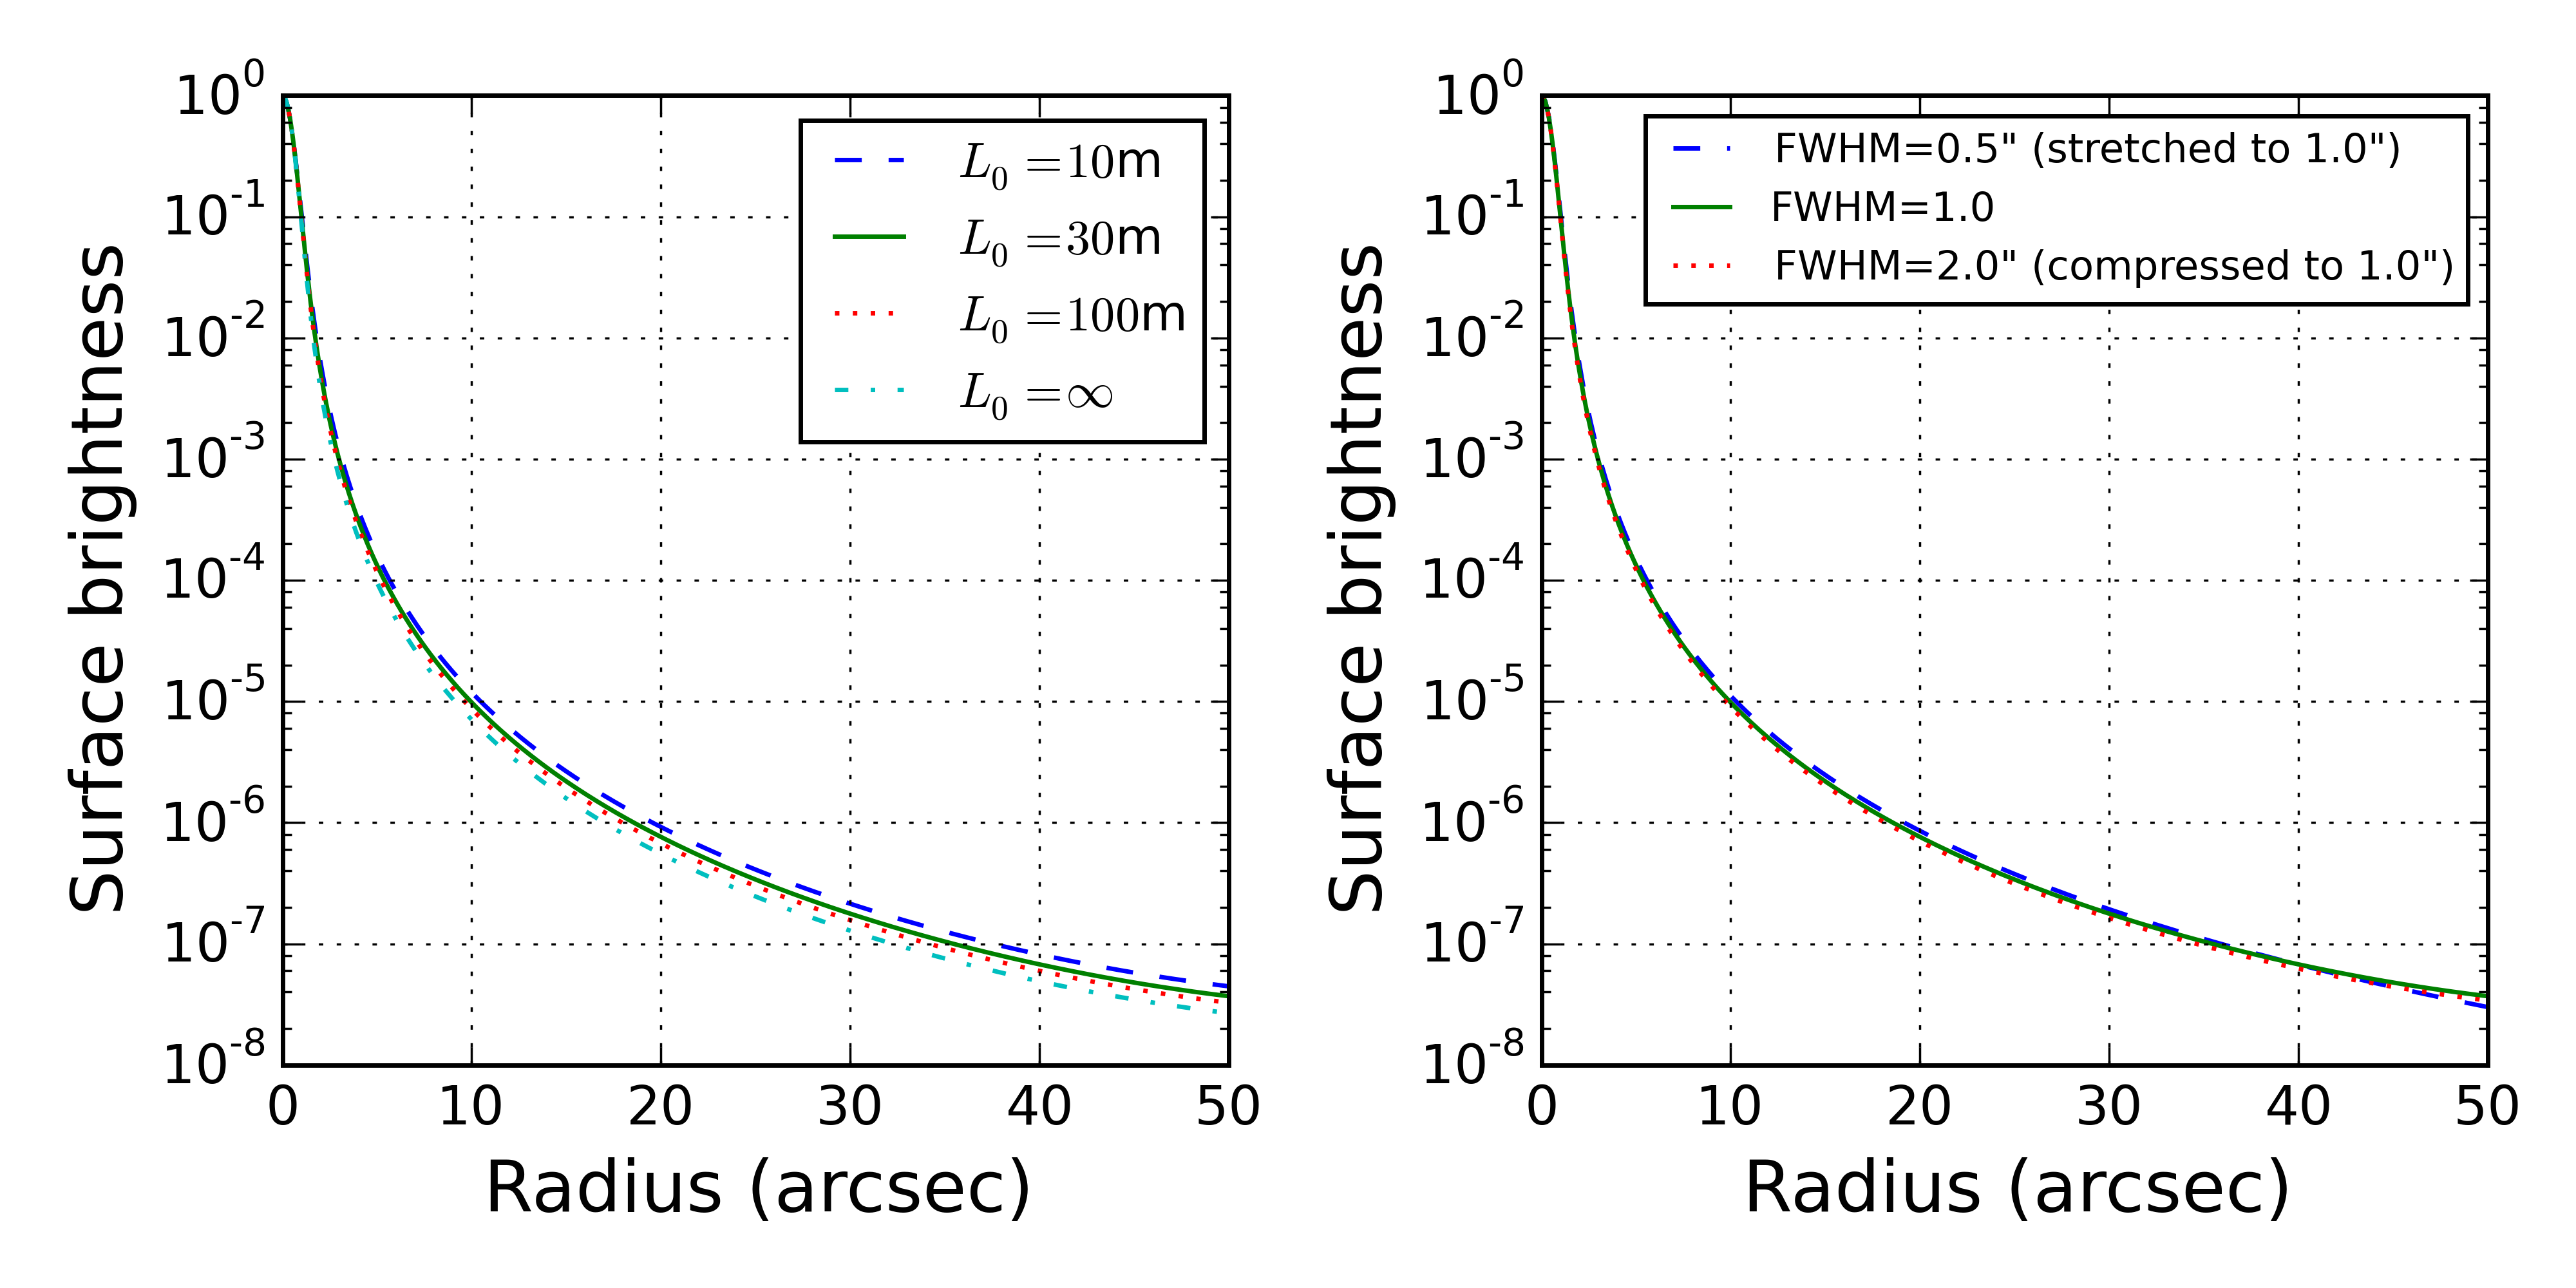
\includegraphics[width=0.8\textwidth]{FIGURES/vonK.png}
\vskip -0.2in 
\caption{PSF radial profiles with the \vk~model for a few different
  outer scale ($L_0$) values. All profiles have FWHM of 1 arcsec, and
  are normalized to unit peak intensity. The \vk~model becomes
  Kolmogorov when $L_0 = \infty$.
\label{fig:vonK}}
\end{figure}




Although the fitted
curves agree with the input data points very well, generally much better than the
original 6-parameter double-Gaussian fit by SDSS, they do not always describe
the PSF tail beyond $\sim 15$ arcsec radius. This discrepancy is easily understood
because it is well known that the PSF tails in the optical bands can be quite
different due to the properties of the CCDs.
For example, the SDSS $i$-band PSF has ``stronger tails''
because of scattering in the CCD.  The Si is transparent at long $i$-band wavelengths 
so light goes all the way through the chip and is reflected off the solder, and passes 
back up through the Si. This effect is not visible in the $z$-band because in this case
thick front-side chips are used (in all other bands, thin back-side chips are used). 



\subsection{Instrumental PSF \label{sec:instrPSF}} 

To improve the fit quality at large radii, in the second fitting step we introduce an
empirical instrumental PSF, so that the observed PSF can be expressed as
a convolution of the atmosphere, represented by the \vk, and
the instrumental PSF,
\begin{equation}
        \textrm{PSF} = \textrm{vonK} (\textrm{FWHM}) \otimes \textrm{PSF}_{\textrm{inst}},
\end{equation} 
where vonK is the \vk~shape, whose only parameter is its FWHM, and
\begin{equation}
        \textrm{PSF}_{\textrm{inst}} = \exp(-\frac{r^2}{2\sigma^2}) + 10^{\eta(ar^2+br+c)}.
\label{eq:psfinst}
\end{equation} 
The standard deviation of the central Gaussian, $\sigma$, cannot be
too wide because the \vk~term already well describes the core of the PSF.
On the other hand, if $\sigma$ is close to zero, once the
total intensity of the instrumental PSF is normalized to 1, too much
widening power would be given to the instrumental PSF tail.
We found that $\sigma = 0.1$ arcsec is an acceptable choice for all the fits.
Because the shape of the instrumental PSF tail should not vary with
time, the parameters $a$, $b$, and $c$ in Eq.~(\ref{eq:psfinst}) are
fixed for each band-camera-column combination.
Their values come from a one-time fit using the same PSF functions,
but with $a$, $b$, and $c$ as additional free parameters.
We used here run 94, field 11 for these one-time fits, but verified that 
the results are stable for other choices of run and field. 
These fits are very slow but need to be done only once.
The best-fit values of $a$, $b$, and $c$ are listed in Table~\ref{tab:abc}.
Although this second fitting step involves a 2-dimensional convolution,
there is only one free parameter in the fit: $\eta$, the normalization of the
instrumental PSF tail. Each two-step PSF fit can be done in a few seconds.

Fig.~\ref{fig:psffit} shows the results of our PSF fits from run 4874. The two-parameter
best fits describe the PSF profiles quite well, both in the core and in the tails. There are 
a total of 108 runs in the SDSS Stripe 82 dataset. Among them, run 4874 is the longest, 
with 981 fields. In the rest of this paper, whenever we illustrate results from a single run, 
we always use run 4874 as the fiducial example run. 


\begin{figure}[th]
\centering
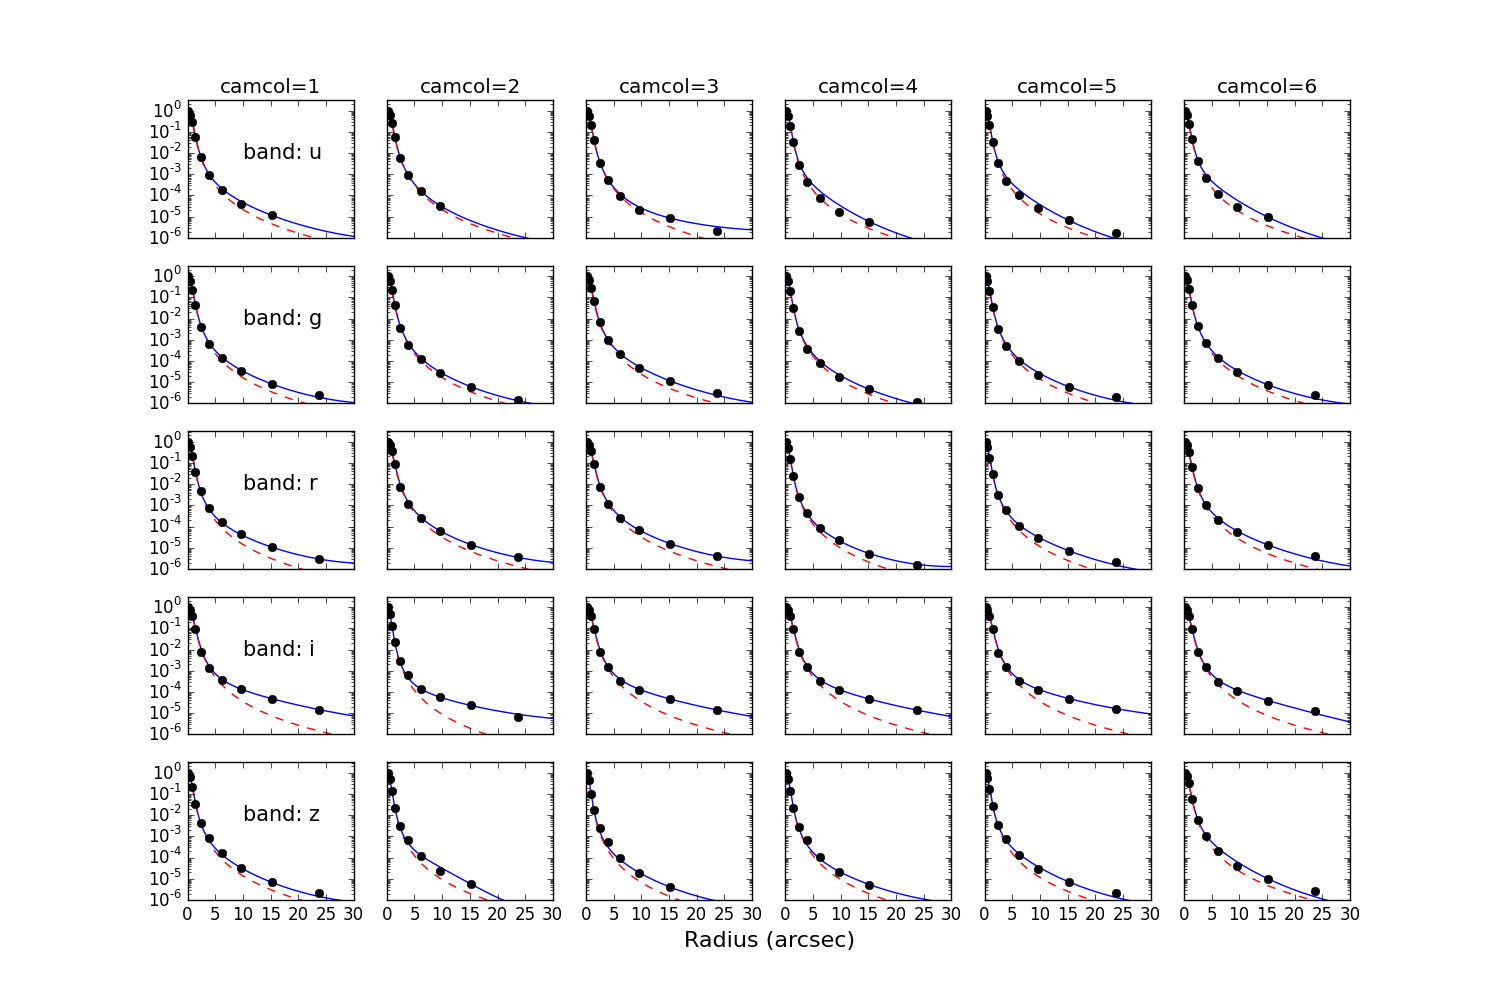
\includegraphics[width=1.0\textwidth]{FIGURES/psffit.png}
\vskip -0.3in
\caption{Fits to the PSF profiles from run 4874, field 21. Symbols are SDSS data. 
  Red dashed curves are the best one-parameter \vk~fits. Blue curves are the red
  curve convolved with the instrumental PSF, where the scaling factor (normalization) 
  for the tail component is allowed to vary. The addition of the instrumental PSF 
  significantly improves the fit quality, especially in the $i$-band. Note that the y-axis 
  is shown on the logarithmic scale.
\label{fig:psffit}}
\end{figure}


\begin{table}[th]
\begin{center}
\caption{Values for instrumental PSF shape parameters $a$, $b$, and $c$.\label{tab:abc}}
\begin{tabular}{c|c|rrrrrr}
\tableline\tableline
\multicolumn{2}{c|}{} & \multicolumn{6}{c}{Camera Column} \\\cline{3-8}
\multicolumn{2}{c|}{} & 1 & 2 & 3 & 4 & 5 & 6\\\hline
   & a($\times 10^{-3}$) & 2.2 & 2.2 & 1.1 & 2.2 & 2.2& 2.2\\
 $u$& b($\times 10^{-1}$) & $-$1.7 & $-$1.7& $-$7.7 & $-$2.3 &$-$2.3 & $-$2.3\\
   & c                             & $-$5.0 & $-$5.0& $-$6.0 & $-$5.0 & $-$5.0&$-$5.0 \\ \hline
  & a($\times 10^{-3}$) & 2.7 & 2.7 & 2.2 & 2.2 & 2.7&2.7 \\
 $g$& b($\times 10^{-1}$) & $-$1.7 & $-$1.7 & $-$1.7 & $-$1.7 &$-$1.7 & $-$1.7\\
   & c                             & $-$5.0 & $-$5.0 & $-$5.0& $-$5.0 &$-$5.0 & $-$5.0\\\hline
  & a($\times 10^{-3}$) & 2.4 & 2.4 & 2.4 & 2.9 &2.2 & 2.2\\
 $r$& b($\times 10^{-1}$) & $-$1.6 & $-$1.6 & $-$1.6 & $-$1.6 &$-$1.7 & $-$1.7\\
   & c                             & $-$5.0 & $-$5.0 & $-$5.0& $-$5.0&$-$5.0 & $-$5.0\\\hline
  & a($\times 10^{-3}$) & 0.7 & 1.1& 0.7 & 0.7 & 0.8& 0.2\\
 $i$& b($\times 10^{-1}$) & $-$0.8 & $-$0.9 & $-$0.8 & $-$0.8 &$-$0.9 & $-$0.8\\
   & c                             & $-$5.0 & $-$5.0 & $-$5.0 & $-$5.0 &$-$5.0 & $-$5.0\\\hline
  & a($\times 10^{-3}$) & 3.1 & $-$2.2 & 3.1 & 2.2 &3.1 & 2.2\\
 $z$& b($\times 10^{-1}$) & $-$2.0 & $-$1.0 & $-$2.0 & $-$1.5 &$-$2.2 & $-$2.3\\
   & c                             & $-$5.0 & $-$5.0 & $-$5.0 & $-$5.0&$-$5.0 & $-$5.0\\
\tableline
\end{tabular}
\end{center}
\end{table}
